StrainEst:
Here we present a computational approach that uses the available genomic data to reconstruct complex strain profiles from metagenomic sequencing, quantifying the abundances of the different strains and cataloging them according to the population structure of the species

However, to fully exploit the potential of metagenomics in clinical and epidemiological applications, computational techniques able to profile microbial communities at resolution beyond the species level are needed, given the high level of phenotypic and genomic variability between strains of the same species4.

Marker-based computational methods:  Despite being able to reach strain-level sensitivity7,8,9, these approaches rest on the implicit assumption that a single dominant strain is present for each species, while it has been shown that the human associated microbiota is often a complex mixture of closely related strains of the same species
1. Segata, N. et al. Metagenomic microbial community profiling using unique clade-specific marker genes. Nat. Methods 9, 811–814 (2012).
2. Wood, D. E. & Salzberg, S. L. Kraken: ultrafast metagenomic sequence classification using exact alignments. Genome Biol. 15, R46 (2014).

Luo, C. et al. ConStrains identifies microbial strains in metagenomic datasets. Nat. Biotechnol. 33, 1045–1052 (2015).

\textbf{StrainEst} The general process of As shown in the image below, in step a), the pairwise Mash distances are computed between with genomes of the species of user interest (G1, G2,…) and the species representative (SR). The genomes with Mash distances >0.1 from the SR are excluded. The choice of 0.1 makes sure that unrelated genomes are discarded, whereas divergent strains from highly variable species are retained. And mash distances were computed with the Mash software, a recent alignment-free tool which outputs a complete pairwise distance matrix for large-sequence data sets. Next, a complete linkage hierarchical clustering is implemented with the remaining genomes using the distances computed in the previous step, in order to remove redundant sequences. For each cluster, the genome with the lowest average distance from the other genomes in the cluster is chosen as a representative (R1, R2,…). And therefore, highly similar, highly related genomes or re-sequencing of strains are represented by a single genome. In step b), the representative sequences are mapped against SR obtaining MR using nucmer package. And ambiguous mappings are removed. In step c), for each representative, the positions of the variant sites (P1, P2,…) are identified and the SNV profiles are extracted. The profiles are clustered at 99 percent identity to guarantee their representativeness. At step d), to create a reference set for metagenomic reads alignments that takes into account the variability of the species, representative genomes are selected for the metagenome alignment step (A1, A2, …) and (e) mapped against SR. f For each metagenome (MG), the reads are aligned to the chosen genomes using Bowtie 2 (Langmead B,  Salzberg SL. Fast gapped-read alignment with Bowtie 2, Nat. Methods, 2012, vol. 9 (pg. 357-359)). g The frequencies of the allelic variants at the variant positions defined in step (c) are extracted from the BAM file; sites with low coverage are filtered according to user-defined filtering parameters; the relative abundance profile is finally inferred by Lasso regression.  \cite{Albanese2017} 

\textbf{Sigma} Firstly, in order to align metagenomic reads onto reference genome, Sigma adopted a short-read alignment algorithm, Bowtie 2 \cite{LangmeadSalzberg2012} by default. Then, Sigma uses stochastic probabilistic model to represent the process of metagenomic sequencing, with z base-pairs of mismatches and a constant probability of σ (5 percent as default) for every mismatch between a read and a genome. The mismatches might be due to genome variability or sequencing errors. And l stands for the length of every read (r), while U stands for the maximum number of mismatches allowed in the read alignment. 
\begin{figure}
    \centering
    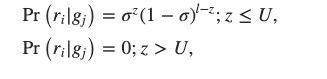
\includegraphics[width=12cm]{Images/sigma1.png}
    \label{fig:sigma1.png}
\end{figure}
Q is the matrix which includes $Pr(r_i|g_j)$ between each read and each genome according to their alignment.
\begin{figure}
    \centering
    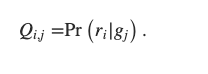
\includegraphics[width=12cm]{Images/sigma2}
    \label{fig:sigma2.png}
\end{figure}
To estimate $Pr(g_j)$, Sigma uses Maximum Likelihood Estimate to maximize the joint probability of all reads, as shown in the figure below.
\begin{figure}
    \centering
    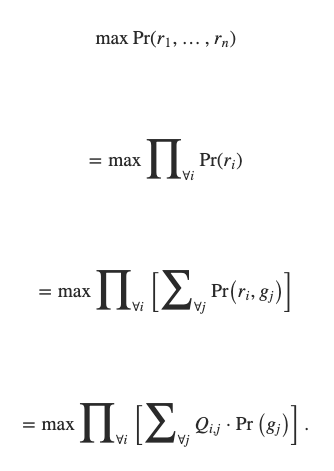
\includegraphics[width=12cm]{Images/sigma6}
    \label{fig:sigma6.png}
\end{figure}
For the sake of precise numeric calculation, Sigma transforms the above formula into log and linear scaling of Q. And therefore, it becomes an optimization problem below, while $G=[G_1,…,G_m]=[Pr(g_1),…,Pr(g_m)]$ for m genomes. To solve the optimization problem, Sigma adopts the NLP method implemented in the Ipopt library (Wachter and Biegler, 2006 ). In their methods, global optimum solutions hold for convex objective functions, while the convexity of Sigma’s objective function is proved. Therefore, Sigma can give maximum likelihood estimates of G. 
\begin{figure}
    \centering
    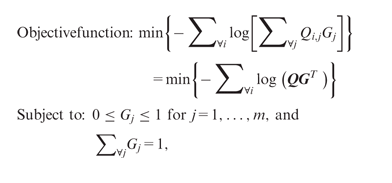
\includegraphics[width=12cm]{Images/sigma7}
    \label{fig:sigma7.png}
\end{figure}
A genome's relative abundance is calculated by the formula below, where θ is the proportion of all aligned reads compared to all sequenced reads.
\begin{figure}
    \centering
    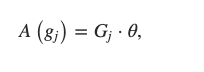
\includegraphics[width=12cm]{Images/sigma3.png}
    \label{fig:sigma3.png}
\end{figure}
Sigma calculates the percentile bootstrap confidence intervals for G, in order to measure the uncertainty caused by the stochastic sampling process of metagenomic sequencing.   A total of B bootstrap resamples (default: 1000) are generated and Sigma calculates MLEs from the bootstrap resamples: $G_1,…,G_B$ , where $G_k=[G_1,k,…,G_m,k]$ . Let $T_j$ be the quantile function for all bootstrap estimates of $G_j$ , i.e. $[G_j,1,…,G_j,B]$. The (1 - $\alpha$) confidence interval of $G_j$ is calculated as below.  The confidence interval of $G_j$ is converted to the confidence interval of its relative abundance, $A(g_j)$ , using the equation in sigma3.png.
\begin{figure}
    \centering
    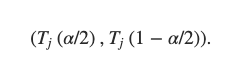
\includegraphics[width=12cm]{Images/sigma4.png}
    \label{fig:Images/sigma4.png}
\end{figure}
Sigma performs hypothesis testing on the null hypothesis that gj is not present. The likelihood ratio test is used for the hypothesis testing, which compares the maximum likelihood of the data under the null hypothesis versus that under the alternative hypothesis. The likelihood ratio is small if the data strongly supports alternative hypothesis. The likelihood ratio test calculates a P -value by assuming a χ2 distribution with one degree of freedom for the statistic, -$2\ln$Λ . The statistical significance of an identified genome is determined not only by its $G_j$ , but also by the distinctness of the genome in the database.
\begin{figure}
    \centering
    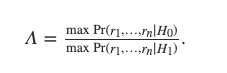
\includegraphics[width=12cm]{Images/sigma5.png}
    \label{fig:Images/sigma5.png}
\end{figure}
